\documentclass{llncs}
\usepackage{standalone}

%\usepackage{acl2012}
%\usepackage{times}
\usepackage{latexsym}

\usepackage[final]{microtype}
\usepackage{flushend}

\usepackage[author={Lyndon White}]{pdfcomment}

\usepackage[boxed]{algorithm2e}


\usepackage{verbatim}
\usepackage{grffile}
%\usepackage[draft]{graphicx}

\usepackage{pgfplots}
\pgfplotsset{compat=1.12}
\usepackage{booktabs, array} % Generates table from .csv
\usepackage{pgfplotstable}

\usepackage{tikz}
\usetikzlibrary{positioning}


%%%%%%%%%%MATH
%\usepackage{amsthm}
\usepackage{amsmath}
\usepackage{amssymb}
\usepackage{amsfonts}

%\theoremstyle{plain}
%\newtheorem{thm}{\protect\theoremname}
%\theoremstyle{definition}
%\newtheorem{defn}[thm]{\protect\definitionname}
%\usepackage{csquotes}
%\usepackage[english]{babel}
%\providecommand{\definitionname}{Definition}
%\providecommand{\theoremname}{Theorem}
%%%%%



%\hypersetup{draft} %Avoid hyperef causing issuse when links broken over pages by disabling hyperref

\usepackage[backend=bibtex,
 style=authoryear-icomp,
 bibencoding=ascii,
 maxcitenames=2,
 url=false,
 hyperref=false
]{biblatex}
\bibliography{master}

\usepackage{cleveref}


%End Packages

\begin{comment}
%%%%%%%%%%%%%%%%%%%%%% Magic Float Layer Fix Settings 
\renewcommand{\topfraction}{.85}
\renewcommand{\bottomfraction}{.7}
\renewcommand{\textfraction}{.15}
\renewcommand{\floatpagefraction}{.66}
\renewcommand{\dbltopfraction}{.66}
\renewcommand{\dblfloatpagefraction}{.66}
\setcounter{topnumber}{9}
\setcounter{bottomnumber}{9}
\setcounter{totalnumber}{20}
\setcounter{dbltopnumber}{9}

%%%%%%%%%%%%%%%%%
\end{comment}


\DeclareMathOperator*{\argmin}{argmin}

%%%%%%% Tables
\newcolumntype{C}[1]{>{\centering\arraybackslash}m{#1}}

\pgfplotstableset{percent style/.style=}
		}},
		%
		%
		every head row/.style={after row=\midrule},
	}
%\usepgfplotslibrary{colorbrewer}
%%%%%%



%opening
\title{Generating Bags of Words from the Sums of their Word Embeddings}
\author{}
\graphicspath{{./figs/}}
\setlength\itemsep{2mm}
\begin{document}

\maketitle

\begin{abstract}
Converting a sentence to a meaningful vector representation has uses in many NLP tasks, however very few methods allow the words to be recovered from that sentence representation. Being able to generate sentences from the vector representations is expected to open up many new applications. As a partway step towards this, we introduce a method for moving from sum of word embedding representations back to the bag of words for the original sentences. This is done using a greedy algorithm to convert the vector to a bag of words. To our knowledge this is the first such work. It demonstrates qualitatively the ability to recreate the words from a large corpus based on its sentence embeddings.
As well as practical applications for allowing classical information retrieval methods to be combined with more recent methods using the sums of word embeddings, the success of this method has theoretical implications on the degree of information maintained by the sum of embeddings representation. This lends some credence to the consideration of the sum of word embeddings as a dimensionality reduced, and meaning enhanced, data manifold for the bag of words.  
\end{abstract}

\section{Introduction} \label{intro}


The task being tackled here is the \emph{resynthesis} of bags of words (BOW) from vector representations. In particular the generation of BOWs from vectors based on the sum of their constituent words' embeddings. It has not received a lot of attention.

The motivations for this work remain the same as in the first work in the related area on sentence generation. \textcite{Dinu2014CompositionalGeneration} observe that from a theoretical perspective given that a sentence encodes its meaning, and the vector encodes the same meaning, then it must be possible to translate in both directions between the natural language and the vector representation. A subset of this is the unordered case, rather than true sentences, which we tackle in this paper. The success of the implementation does demonstrate the truth of this dual space theory, for the unordered cases considered. There are also some potential practical applications of such an implementation, often ranging around certain types of ``translation'' tasks.

Given suitable bidirectional methods for converting between sentence vectors and bags of words, the sentence vector space can be employed as a \emph{lingua franca} for translation between various forms of information -- though with loss of word order information. The most obvious of which is literal translation between different natural languages; however the use extends beyond this.

Several approaches have been developed for representing images and sentences in a common vector space. This is used to select a suitable caption a list of candidates \parencite{farhadi2010every,socherDTRNN}. Similar methods, creating a common space between images and SOWE of the keywords describing them, could be used to generate keyword descriptions using BOW resynthesis -- without any need for a list. This would allows classical word-based information retrieval and indexing techniques to be applied to images.

Another similar use is the replacement of vector based extractive summarisation \textcite{KaagebExtractiveSummaristation,yogatamaextractive}, with abstractive summarisation. Again generating a keyword summary from a document or a paragraph. The promising use of BOWE generation for all these applications is to have a separate model trained to take the source information (e.g. a picture for image description, or a cluster of sentences for abstract summarisation) as its input and train it to output a SOWE vector which can then be used to generate the sentence.

\begin{comment}
There are currently three existing methods for sentence regeneration -- each tied to different machine learnt embedding representation. 
The current state of the art for full sentence generation are the works of \cite{iyyer2014generating} and \cite{Bowman2015SmoothGeneration}. 
Beyond the original work in the area of \cite{Dinu2014CompositionalGeneration} which is only theorised to extend beyond short phrases, both produce full sentences. These sentences are qualitatively shown to be loosely similar in meaning to the original sentences. Neither works has produced quantitative evaluation, making it hard to determine between them. Both are detailed further in the next section.
\end{comment}

The method proposed in this paper takes in a sum of word embeddings (SOWE) sentence vector, and outputs the bag of word (BOW) which it corresponds to. The input is a vector for example $\tilde{s}=[0.11, 0.57,-0.21,...,1.29]$, which approximates a SOWE vector, and outputs a BOW for example \texttt{\{, : 1,best: 1, worst: 1, it: 2, of: 2, the: 2, times: 2, was: 2\}} -- the BOW for the opening line of Dickens' \emph{Tale of Two Cities}. That input vector could come direct as the SOWE representation of a reference sentence (as is the case for the evaluation of our method presented in this paper). More practically it could come as the output of some other process; for example a machine learnt mapping from an image to the vector representation of its textual description. This vector representation is transformed through our process into a human readable sentence.

The sentence generation is done in two steps, as shown in \Cref{block_diagram}. The first step is to determine which words are in the sentence -- this converts the SOWE embedding into a bag of words. The second step is to order that bag of words into a sentence -- a language modelling task. This paper will focus on the first part -- the word selection problem. A demonstration of the feasibly of solving the second part -- the ordering problem --  is shown in \Cref{ordering}.

\begin{figure}
	\centering 
	\documentclass{standalone}

\usepackage{tikz}
\usetikzlibrary{positioning}


\begin{document}

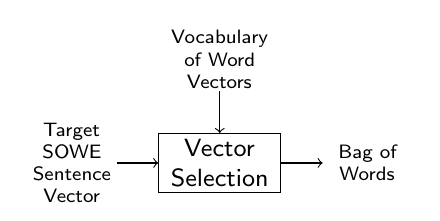
\begin{tikzpicture}[
	every node/.style={ text width=4em,
    					align=center,
                        font=\scriptsize\sffamily,
                        inner sep=1pt
                        },
	proc/.style= {draw,
    			  font=\small\sffamily,
                  inner sep = 2pt
    }
]
	\node (input) [inner sep=-4pt] {Target SOWE Sentence Vector};
    \node (selection) [proc, right = 1.5em of input]{Vector\\ Selection};
	\node (vocab) [above = 1.5em of selection]{Vocabulary of Word Vectors};
    \node (output) [inner sep=-4pt, right=1.5em of selection] {Bag of Words};
    \draw[->] (input) -- (selection);
    \draw[->] (vocab) -- (selection);
    \draw[->] (selection) -- (output);
\end{tikzpicture}

\end{document}
	\caption{The process for the regenerating sentences from SOWE-type sentence vectors. \pdfcomment{Update diagram to refer to the input as the target vector}}
	\label{block_diagram}
\end{figure}

The rest of the paper is organized into the following sections. \Cref{relwork} introduces the area, discussing in general sentence models, and prior work on generation. \Cref{framework} explains the problem in detail and our algorithm for solving it. \Cref{evalsettings} described the settings used for evaluation. \Cref{results} presents the results on this evaluation. The paper concluded with \Cref{conclusion} and a discussion of future work on this problem.


\section{Background}\label{relwork}


Bag of words is an traditional method for representing a text, sentence or document, used in information retrieval. The text is replaced with an unordered multiset of how often each word occurs -- often represented as a vector of the counts of each word in the vocabulary. 

Word embeddings are vector representations of words. They have been shown to encode important syntactic and semantic properties. There are many different methods for generating various types of word vectors \cite{Yin2015}. Two of the more notable are the continuous bag of words and skip gram of the \texttt{word2vec} method of \cite{mikolov2013efficient,mikolov2013linguisticsubstructures} and the Global Vector word representations (GloVe) of \cite{pennington2014glove}. The evaluations presented in this paper use GloVe, though preliminary experiments have found similar results using \texttt{word2vec}. Beyond word representations are sentence vectors. 


Sentence vectors represent sentences -- they are often derived from word vectors. Like word vectors they can capture semantic and syntactic features. Sentence vector creation methods include the works of \textcite{le2014distributed} and \textcite{socher2014recursive}. Far simpler than those methods, is the  sum of word embeddings (SOWE). SOWE (like BOW) draws significant criticism for not only disregarding sentence structure, but disregarding word order entirely when deriving to sentence vector. However this weaknesses, while valid, may be offset by the improved discrimination allowed through words directly affecting the sentence vector -- without the potential information loss through the indirection of more complex methods. This may allow to be comparable overall to the more linguistically consistent compositional embeddings when it come to representing sentence meaning. 


Recently \textcite{White2015SentVecMeaning} found that when classifying real-world sentences into groups of semantically equivalent paraphrases, that using SOWE as the input resulted in very accurate classifications. In that work White et. al. partitioned the sentences into groups of paraphrases, then evaluated how well a linear SVM could classify unseen sentences into the class given by its meaning. They tested this using a variety of different sentence embeddings techniques as input to the classifier. They found that the classification accuracy when using SOWE as the input very similar to that of the best performing methods -- less that 0.6\% worse on the harder task. From this they concluded that the mapping from the space of sentence meaning to the vector space of the SOWE, resulted in sentences with the same meaning going to distinct areas of the vector space.

\textcite{RitterPosition} presents a similar task on spacial-positional meaning, which used carefully constructed artificial data, for which the meanings of the words interacted non-simply -- thus favouring the compositional models. In their evaluation the task was classification with a Naive Bayes classifier into one of five categories of different spatial relationships. Here also SOWE was found performing comparably and again even out performing the compositional models. The best of the SOWE models they evaluated, outperformed the next best model (compositional or otherwise) by over 5\%. These results suggest this simple method is still worth consideration. SOWE is the basis of the work presented in this paper.

\section{The Vector Selection Problem}

At the core of this problem is what we will call the Vector Selection Problem, to select which word vectors from  will sum to be closest to the target SOWE. The word vectors come from a known vector vocabulary, and are selected with potential repetition.
As there is a one to one correspondence between the vector word embeddings and their words, solving for the word embeddings used provides a unique solution to this. This relies on no two words having exactly the same embeddings -- which is true for all current word embedding techniques.

\renewcommand{\c}{\tilde{c}}
\newcommand{\s}{\tilde{s}}
\newcommand{\x}{\tilde{x}}
\renewcommand{\t}{\tilde{t}}
\newcommand{\N}{\mathbb{N}}
\newcommand{\R}{\mathbb{R}}
\newcommand{\V}{\mathcal{V}}

%\begin{defn}{The Vector Selection Problem}
\begin{definition}{The Vector Selection Problem}
	is defined on $(\V, \s,\,d)$ \\for a finite vocabulary of vectors $\V$, $\V\subset{\R}^{n}$, a target sentence vector $ \s$, $ \s\in\R^{n}$, and any distance metric $d$, by:
		\[
		\argmin_{\left\{ \forall\c\in\N_{0}^{V}\right\} }\:d( \s,\,\sum_{\x_j\in\V}\:\x_{j}c_{j})
		\]
						
		$\x_{j}$ is the vector embedding for the jth word in the vocabulary
		$\x_{j}\in\V$ and $c_j$ is the jth element of the count vector $\c$ being optimised -- it is the count of how many times the $x_j$ occurs in approximation to the sum being assessed; and correspondingly it is the count of how many times the jth word from the vocabulary occurs in the bag of words.
		The selection problem is thus finding the right words with the right multiplicity, such that the sum of their vectors is as close to the input target vector, $\s$, as possible.
\end{definition}
%\end{defn}

\subsection{NP-Hard Proof}
The vector selection problem is NP-Hard. It is possible to reduce from any given instance of a \emph{subset sum problem} to a vector selection problem. The \emph{subset sum problem} is NP-complete \parencite{karp1972reducibility}. It is defined: for some set of integers ($\mathcal{S}\subset\mathbb{Z}$), does there exist a subset ($\mathcal{L}\subseteq\mathcal{S}$) which sums to zero ($0=\sum_{l_i\in \mathcal{L}} l_i$).  A suitable metric, target vector and  vocabulary of vectors corresponding to the elements $\mathcal{S}$ can be defined by a bijection; such that solving the vector selection problem will give the subset vectors corresponding a subset of $\mathcal{S}$ with the smallest sum; which if zero indicates that the subset sum does exists, and if nonzero indicates that no such subset ($\mathcal{L}$) exists. A fully detailed proof of the reduction from subset sum to the vector selection problem can be found on the first author's website.\footnote{[[URL removed for blinding.]]}

\subsection{Selection Algorithm}
The algorithm proposed here to solve the selection problem is a greedy iterative processes that continues to convergence. It is a fully deterministic method, requiring no training, beyond having the word vector mapping provided. In each iteration, first a greedy search (Greedy Addition) for a path to the targeted sum point $\s$ is done, followed by correction with a substitution based step (n-Substitution). This process is repeated until no change is made to the path. The majority of the selection is done in the Greedy Addition step, while the substitution is handles fine tuning. 

\subsubsection{Greedy Addition}
The greedy addition step is characterised by adding the best vector to the bag at each step (see the pseudo-code in \Cref{pseudocode:greedyaddition}). At each step, all the vectors in the bag are summed, and each vector in the vocabulary is added in turn to evaluate the new distance the new bag would have from the target, if any of the new bags are closer than the existing bag, then the best of them replaces the existing bag. This continues until there is no option to add any of the vectors without moving the sum away from the target. Greedy addition works surprisingly well on its own, but it is enhanced with a fine tuning step to decrease its greediness.

\begin{algorithm}
	\SetAlgoLined
		\KwData{the metric $d$\\the target sum $\s$\\ the vocabulary of vectors $\V$\\The current best bag of vectors $bag_c$: initially $\emptyset$}
		\KwResult{The modified $bag_c$  which sum to be as close as greedy search can get to the target $\s$, under the metric $d$}
		\Begin{
		$\t \longleftarrow \sum\limits_{x_i\in bag_c} x_i$\;

		\While{true}{
			$\x^\ast \longleftarrow \argmin\limits_{x_j\in \V} d(\s, \t+\x_j) $\;
			
			\eIf{$d(\s, \t+\x^\ast)  < d(\s, \t)$}{
				$t \longleftarrow \t + \x^\ast$\;
				$bag_c \longleftarrow bag_c \cup \{\x^\ast\}$\;	
			}{
				\tcc{No further improving step found}
				\Return{$bag_c$} 
			}
		}
		
	}
\caption{GreedyAddition. In practical implementation, the bag of vectors can be represented as list of indexes into columns of the embedding vocabulary matrix}
\label{pseudocode:greedyaddition}
\end{algorithm}


\subsubsection{n-Substitution}
We define a new substitution based method for fine tuning solutions called n-substitution. It can be described as considering all subbags containing up to $n$ elements, consider replacing them with a new sub-bag of up that size from the vocabulary, including none at all, if that would result in getting closer to the target $\s$. 

The reasoning behind performing the n-substitution is to correct for greedy mistakes. Consider the 1 dimensional case where $\V={24,25,50}$ and $\s=98$, $d(x,y)=\left|x-y\right|$. Greedy addition would give  $bag_c=[50,25,24]$ for a norm-distance of $1$, but a perfect solution  is $bag_c=[50,24,24]$ which is found using  substitution. This substitution method can be looked at as re-evaluating past decisions in light of the future decisions. In this way it lessens the greed of the addition step. 

The n-substitution step has time complexity $O(\binom{C}{n}V^n)$ operations -- for $C=\sum \c$ i.e. current cardinality of $bag_c$. With large vocabularies it is only practical to consider 1-substitution. With the Brown Corpus, where $V\approxeq 40,000$, was found that 1-substitution provides a significant improvement over greedy addition alone. On a smaller trial corpora, where $V\approxeq 1,000$, 2-substitution was used and found to give further improvement. In general it is possible to initially use 1-substitution, with the overall algorithm, and if the algorithm converges to a poor solution (i.e. nonzero distance to target in the evaluation trials), then the selection algorithm can be retired from the converged solution, using 2-substitution and so forth. As $n$ increases the greed decreases; at the limit the overall algorithm is not greedy at all, but is rather an exhaustive search.



\section{Experimental Setup and Evaluations} \label{evalsettings}


\subsection{Word Embeddings}
GloVe representations of words are used in our evaluations \parencite{pennington2014glove}. There are many varieties of word embeddings which function with our algorithm. GloVe was chosen simply become of the availability of a large pre-trained vocabulary of vectors. The representations used for evaluation were pretrained on pre-trained on 2014 Wikipedia and Gigaword 5\footnote{Kindly made available online at \url{http://nlp.stanford.edu/projects/glove/}}. Preliminary results with \texttt{word2vec} suggest that those representations perform similarly.

\subsection{Corpora}

The evaluation was performed on the Brown Corpus \parencite{francis1979brown} and a subset of the Books Corpus \parencite{moviebook}. The Brown Corpus was  sourced with samples from a 500 fictional and non-fictional works from 1961. The Books Corpus was sourced from 11,038 unpublished booked. The Books Corpus is extremely large, containing roughly 74 million sentences. After preprocessing we randomly selected ~0.1\% of these for evaluation.

For simplicity of evaluation, sentences containing words not found in the vector vocabulary are excluded. These were generally rare mis-spellings and unique numbers (such as serial numbers). In general it is of-course possible to simply to have trained a set of vocabulary of word vectors including those words. Similarly, words which are not used in the corpus are excluded from the vector vocabulary. 

After the preprocessing the final corpora can be described as follows. The Brown Corpus has 42,004 sentences and a vocabulary of 40,485 words. Where as, the Books Corpus had 66,464 sentences, and a vocabulary of 178,694 words. 

\subsection{Vector Selection}
The euclidean metric was used to measure how close potential solutions were to the target vector. The choice of distance metric controls how close each vector is considered to the partial sum during the greedy selection. The commonly used cosine similarity, or the linked angular distance, have an issue of non-zero distances between distinct points -- making them not true distance metrics. For example the SOWE of \emph{So he said `` ``So'' said he.''.} has a zero distance under those measures to \emph{"He said so.''}. However, that example is ungrammatical, and pathological. True metrics such a the euclidean metric used do not have this problem. Further investigation may find other better distance metrics for this step.

The Julia programming language \parencite{Julia}, was used to create the implementation of the method, and the evaluation scripts for the results presented in the next section. These this implementation  and the scripts are available on-line.\footnote{[[URL Blinded for Review]]}

\section{Results and Discussion} \label{results}

\begin{table}
	\pgfplotstabletypeset[col sep=comma,fixed zerofill, precision=3,column type=C{5em},
		columns/Corpus/.style={string type},
		columns/Word Embedding Dimensions/.style={string type},
		columns/Portion Perfect/.style={percent style, precision=1},
		every head row/.style={
	    	after row=\midrule
		}]{data/selection_overall_len_scores.csv}
	\caption{ The performance of the BOW generation method. Note the final line is the Books Corpus, where-as the preceding are the Brown Corpus.}
	\label{table:overall}
\end{table}


\begin{figure}
	\pgfplotstableread[col sep=comma,header=has colnames]{data/selection_len_scores.csv}{\sellenscores}
%	\pgfplotstableread[col sep=comma,header=has colnames]{data/dummy.csv}{\sellenscores}
	\definecolor{colorbrewer1}{RGB}{141,211,199}
	\definecolor{colorbrewer2}{RGB}{255,255,179}
	\definecolor{colorbrewer3}{RGB}{190,186,218}
	\definecolor{colorbrewer4}{RGB}{251,128,114}
	\definecolor{colorbrewer5}{RGB}{128,177,211}
%	\pgfplotscreateplotcyclelist{colorbrewerlist}{}

	\begin{tikzpicture}
	\begin{axis}[xlabel=Ground Truth Sentence Length,
					ylabel=Mean Jacard Index,
					width=12.5cm,height=6cm,cycle list name=exotic]
%	\addplot table [y=a,x=b]{\sellenscores};
	\addplot table [y=brown_glove50_jaccard_mean,x=ground_len]{\sellenscores};
	\addplot table [y=brown_glove100_jaccard_mean,x=ground_len]{\sellenscores};
	\addplot table [y=brown_glove200_jaccard_mean,x=ground_len]{\sellenscores};
	\addplot table [y=brown_glove300_jaccard_mean,x=ground_len]{\sellenscores};%
	\addplot table [y=books_0_01_glove300_jaccard_mean,x=ground_len]{\sellenscores};
	\legend{50D Brown, 1000D Brown, 200D Brown,300D Brown, 300D Books}					
	\end{axis}
	\end{tikzpicture}


	\caption{The mean Jaccard index achieved during the word selection step, shown against the ground truth length of the sentence. Note that the varst majority of sentences are in the far left end of the plot. The Q3 on sentence length is 25 for Brown, and 17 for Books. The diminishing samples is also the cause of the noise, as the ground length increases.}
	\label{figure:exactlenscore}
\end{figure}


\begin{table*}[t!]
	\centering
	INSERT TABLE OF EXAMPLES HERE
	
	\caption{Examples of  }
	\label{table:examples}
\end{table*}


The table shows the performance of our method across both corpora. Five measures are reported. 
The most clear is the portion of exact matches -- this is how often out of all the trials the method producted the exact correct bag of words. The remaining measures are all means across all the values of the measures in each trial.  The Jaccard index is the portion of overlap between the reference BOW, and the output BOW -- it is the cardinality of the intersection divided by that of the union. The precision is the portion of the output words that were correct; and the recall is the portion of all correct words which were output. The $F_1$ score is the harmonic mean of precision and recall.

The recall is higher is than the precision, indicating that the method is tends to produce additional incorrect words (lowering the precision), more often than missing words (which would lower the recall). This aligns with observations that can be made by looking at the examples shown in \Cref{table:examples}. 

Initial investigation focused on the relationship between the number of dimensions in the word vector and the performance. This was carried out on the smaller Brown corpus. Results confirmed the expectation that higher dimensional embeddings allow for better generation of words. The best performing embedding size (i.e. the largest)  was then used to evaluate success on the Books Corpus.

Thought not apparent from the raw results shown in \Cref{table:overall}, performance was worse in on the Books Corpus, due to its larger vocabulary size. The overall results are better in the Books Corpus, however this is due to it having much shorter sentences. As can be seen in \Cref{figure:exactlenscore}, when taken as a function of the sentence length, performance on Books is worse than Brown. We attribute this to the Books Corpus vocabulary being over four times larger -- much more scope for mistakes.




\section{Conclusion} \label{conclusion}
A method was presented for how to regenerate a bag of words, from the sum of a sentence's word embeddings. The word selection problem, of going from the sum of embeddings to the words, is NP-Hard. A greedy algorithm was found to perform well at the task, particularly for shorter sentences when high dimensional embeddings are used. It was also demonstrated that a simple probabilistic language model can be used to order the bag of words output to regenerate the original sentences.

Resynthesis degraded as sentence length increased, but remained strong with higher dimensional models up to reasonable length. It also decreased as the vocabulary size increased, however even the smaller Brown Corpus vocabulary, containing roughly 40,000 words is beyond what is suggested as the necessary  as the vocabulary size for most uses \parencite{nation2006large}.

From a theoretical basis the resolvability of the selection problem shows that adding up the word vectors does preserve the information on which words were used; particularly for higher dimensional embeddings. This shows clearly that collisions do not occur (at least with frequency) such that two unrelated sentences do not end up with the same SOWE representation. 

Future work in this area would be use a stochastic language model to suggest suitable orderings for the bags of words. While this would not guarantee correct ordering every-time, we speculate that it could be used to find reasonable approximations often. Thus allowing this bag of words generation method to be used for full sentence generation, opening up a much wider range of applications.

\printbibliography
	
\end{document}


